\section*{Half-Plane Intersection}

\subsection*{Definitions}

\begin{definition}[half-planes]
A line $l$ on 2D plane with function $y = ax - b$ defines two \emph{half-planes}:
the \emph{upper half-plane}: $y \ge ax -b$ and the \emph{lower half-plane}: $y \le ax -b$.
\end{definition}

\begin{definition}[upper- and lower-envelop]
Let $L = \{y = a_i x - b_i \mid 1 \le i \le n \}$ be a set of lines on 2D plane.
We define the \emph{upper-envelop} of $L$, denoted as $UE(L)$, as the intersection of
the corresponding $n$ upper half-planes $\{y \ge a_i x -b \mid 1 \le i \le n \}$.
We define the \emph{lower-envelop} of $L$, denoted as $LE(L)$, as the intersection of
the corresponding $n$ lower half-planes $\{y \le a_i x -b \mid 1 \le i \le n \}$.
\end{definition}

Either upper-envolop or lower-envelop of a set of lines can be represented
as the list of lines that define its boundary from left to right. In the example
below, we can write $UE(L) = (l_1, l_2, l_4, l_7)$
and $LE(L) = (l_7, l_5, l_1)$.

\begin{figure}[h!]
\centering{\tikzset{every picture/.style={line width=0.75pt}} %set default line width to 0.75pt        

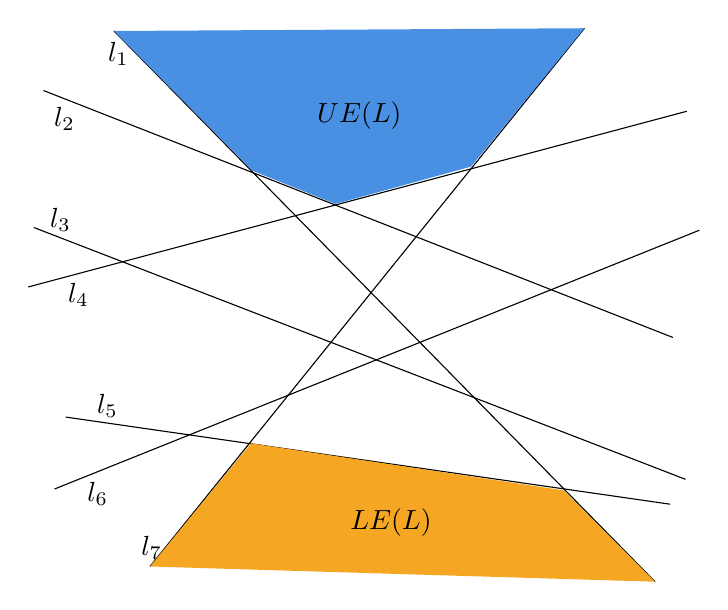
\begin{tikzpicture}[x=0.5pt,y=0.5pt,yscale=-1,xscale=1]
%uncomment if require: \path (0,420); %set diagram left start at 0, and has height of 420

%Straight Lines [id:da8861644180083026] 
\draw    (92.13,398.52) -- (406.13,9.52) ;
%Straight Lines [id:da40732713893670314] 
\draw    (457.13,409.52) -- (66.13,11.52) ;
%Straight Lines [id:da44367949821680464] 
\draw    (468.13,353.52) -- (31.13,290.52) ;
%Straight Lines [id:da2319769205561817] 
\draw    (470,233) -- (15.13,54.52) ;
%Straight Lines [id:da8632177571421473] 
\draw    (480.13,69.52) -- (4.13,196.52) ;
%Straight Lines [id:da43810226035482036] 
\draw    (489.13,155.52) -- (23.13,342.52) ;
%Straight Lines [id:da08264547138329514] 
\draw    (479.13,335.52) -- (8.13,153.52) ;
%Shape: Polygon [id:ds5174786512352558] 
\draw  [draw opacity=0][fill={rgb, 255:red, 74; green, 144; blue, 226 }  ,fill opacity=1 ] (66.13,11.52) -- (406.13,9.52) -- (324.13,109.52) -- (226.13,136.52) -- (166.13,112.52) -- cycle ;
%Shape: Polygon [id:ds7523383015569914] 
\draw  [draw opacity=0][fill={rgb, 255:red, 245; green, 166; blue, 35 }  ,fill opacity=1 ] (391.13,343.52) -- (457.13,409.52) -- (92.13,398.52) -- (165.13,309.52) -- (165.13,309.52) -- cycle ;

% Text Node
\draw (60,17.93) node [anchor=north west][inner sep=0.75pt]  [font=\normalsize] [align=left] {$\displaystyle l_{1}$};
% Text Node
\draw (21,64.93) node [anchor=north west][inner sep=0.75pt]  [font=\normalsize] [align=left] {$\displaystyle l_{2}$};
% Text Node
\draw (18,137.93) node [anchor=north west][inner sep=0.75pt]  [font=\normalsize] [align=left] {$\displaystyle l_{3}$};
% Text Node
\draw (31,191.93) node [anchor=north west][inner sep=0.75pt]  [font=\normalsize] [align=left] {$\displaystyle l_{4}$};
% Text Node
\draw (52,271.93) node [anchor=north west][inner sep=0.75pt]  [font=\normalsize] [align=left] {$\displaystyle l_{5}$};
% Text Node
\draw (45,335.93) node [anchor=north west][inner sep=0.75pt]  [font=\normalsize] [align=left] {$\displaystyle l_{6}$};
% Text Node
\draw (84,374.93) node [anchor=north west][inner sep=0.75pt]  [font=\normalsize] [align=left] {$\displaystyle l_{7}$};
% Text Node
\draw (211,60.93) node [anchor=north west][inner sep=0.75pt]   [align=left] {$\displaystyle UE( L)$};
% Text Node
\draw (235,354.93) node [anchor=north west][inner sep=0.75pt]   [align=left] {$\displaystyle LE( L)$};


\end{tikzpicture}
}
\caption{Illustration of upper-envelop and lower-envelop of lines $L = \{l_1, l_2, \cdots, l_7\}$.}
\end{figure}

We want to design efficient algorithms to calculate the upper- and lower-envelop of a set of lines.
In fact, we don't need to design any new algorithm here. Below we will show that, the problem of finding
upper- and lower-envolop of a set of lines is equivalent to the problem of finding the convex hull
of a set of points. Therefore, the algorithms we've designed for finding the convex hull can be
directly used to find the upper- and lower-envelop of lines.


\subsection*{Duality}

\begin{definition}[dual of a point]
Let $p = (p_x, p_y)$ be a point on 2D plane. We define the \emph{dual} of $p$, denoted as $p^*$, as
a line with function $y = p_x x - p_y$ on 2D plane.
\end{definition}

\begin{definition}[dual of a line]
Let $l$ be a line with function $y = ax-b$ on 2D plane. We define its \emph{dual}, denoted as $l^*$,
as a point with coordinates $(a,b)$ on 2D plane.
\end{definition}

The following three properties are direct consequences of above definitions. (Think how to prove them.)

\begin{property}
For any point $p$, we have $(p^*)^* = p$. 
For any line $l$, we have $(l^*)^* = l$. 
\end{property}

\begin{property}
Point $p$ is on line $l$ if and only if point $l^*$ is on line $p^*$.
\end{property}

\begin{property}
Point $p$ is above~(resp.\ below) line $l$ if and only if point $l^*$ is above~(resp.\ below) line $p^*$.
\end{property}


\subsection*{Half-plane Intersection vs.\ Convex Hull}

\begin{definition}[upper- and lower-hull]
Let $P$ be a set of points, and let $CH(P)$ be the convex hull of $P$.
Let $p_S\in CH(P)$ be the vertex with smallest $x$-coordinate,
and $p_L\in CH(P)$ be the vertex with largest $x$-coordinate.
Therefore $p_S$ and $p_L$ partition $CH(P)$ into two parts:
the list of vertices from $p_S$ to $p_L$ following the counter-clockwise order is called \emph{lower hull} of $P$, denoted as $LH(P)$;
the list of vertices from $p_L$ to $p_S$ following the counter-clockwise order is called \emph{upper hull} of $P$, denoted as $UH(P)$.
\end{definition}

We now show that upper- and lower-envelop of lines is essentially the same with lower- and upper-hull of points.
We first prove the connection between upper-envelop and lower-hull; the other one, i.e., lower-envelop and upper-hull, can be proved symmetrically.

Let $L$ be a set of lines, we define $L^* = \{l^* \mid l \in L\}$, i.e., the set of ``dual points'' of $L$.


\begin{figure}[h!]
\centering{

\tikzset{every picture/.style={line width=0.75pt}} %set default line width to 0.75pt        

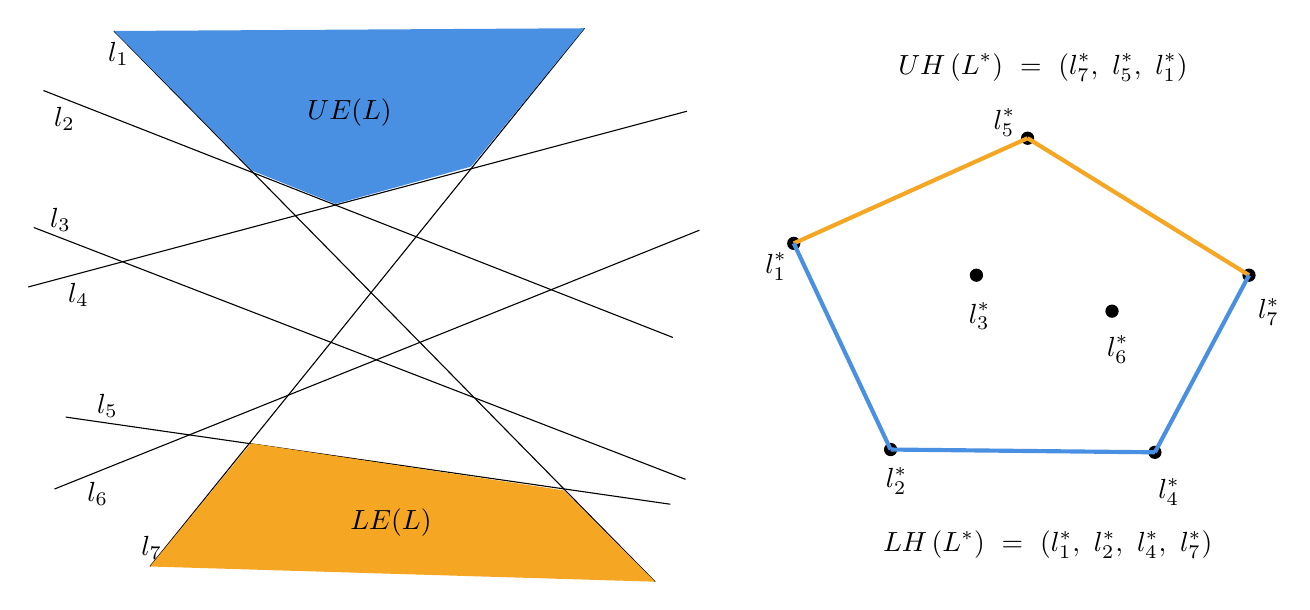
\begin{tikzpicture}[x=0.5pt,y=0.5pt,yscale=-1,xscale=1]
%uncomment if require: \path (0,420); %set diagram left start at 0, and has height of 420

%Straight Lines [id:da8861644180083026] 
\draw    (92.13,398.52) -- (406.13,9.52) ;
%Straight Lines [id:da40732713893670314] 
\draw    (457.13,409.52) -- (66.13,11.52) ;
%Straight Lines [id:da44367949821680464] 
\draw    (468.13,353.52) -- (31.13,290.52) ;
%Straight Lines [id:da2319769205561817] 
\draw    (470,233) -- (15.13,54.52) ;
%Straight Lines [id:da8632177571421473] 
\draw    (480.13,69.52) -- (4.13,196.52) ;
%Straight Lines [id:da43810226035482036] 
\draw    (489.13,155.52) -- (23.13,342.52) ;
%Straight Lines [id:da08264547138329514] 
\draw    (479.13,335.52) -- (8.13,153.52) ;
%Shape: Polygon [id:ds5174786512352558] 
\draw  [draw opacity=0][fill={rgb, 255:red, 74; green, 144; blue, 226 }  ,fill opacity=1 ] (66.13,11.52) -- (406.13,9.52) -- (324.13,109.52) -- (226.13,136.52) -- (166.13,112.52) -- cycle ;
%Shape: Polygon [id:ds7523383015569914] 
\draw  [draw opacity=0][fill={rgb, 255:red, 245; green, 166; blue, 35 }  ,fill opacity=1 ] (391.13,343.52) -- (457.13,409.52) -- (92.13,398.52) -- (165.13,309.52) -- (165.13,309.52) -- cycle ;
%Flowchart: Connector [id:dp46379119482531805] 
\draw  [fill={rgb, 255:red, 0; green, 0; blue, 0 }  ,fill opacity=1 ] (553,165) .. controls (553,162.58) and (554.96,160.62) .. (557.38,160.62) .. controls (559.79,160.62) and (561.75,162.58) .. (561.75,165) .. controls (561.75,167.42) and (559.79,169.38) .. (557.38,169.38) .. controls (554.96,169.38) and (553,167.42) .. (553,165) -- cycle ;
%Flowchart: Connector [id:dp040615914180513246] 
\draw  [fill={rgb, 255:red, 0; green, 0; blue, 0 }  ,fill opacity=1 ] (722,89) .. controls (722,86.58) and (723.96,84.62) .. (726.38,84.62) .. controls (728.79,84.62) and (730.75,86.58) .. (730.75,89) .. controls (730.75,91.42) and (728.79,93.38) .. (726.38,93.38) .. controls (723.96,93.38) and (722,91.42) .. (722,89) -- cycle ;
%Flowchart: Connector [id:dp7594591399684455] 
\draw  [fill={rgb, 255:red, 0; green, 0; blue, 0 }  ,fill opacity=1 ] (814,316) .. controls (814,313.58) and (815.96,311.62) .. (818.38,311.62) .. controls (820.79,311.62) and (822.75,313.58) .. (822.75,316) .. controls (822.75,318.42) and (820.79,320.38) .. (818.38,320.38) .. controls (815.96,320.38) and (814,318.42) .. (814,316) -- cycle ;
%Flowchart: Connector [id:dp3930810481617427] 
\draw  [fill={rgb, 255:red, 0; green, 0; blue, 0 }  ,fill opacity=1 ] (623,314) .. controls (623,311.58) and (624.96,309.62) .. (627.38,309.62) .. controls (629.79,309.62) and (631.75,311.58) .. (631.75,314) .. controls (631.75,316.42) and (629.79,318.38) .. (627.38,318.38) .. controls (624.96,318.38) and (623,316.42) .. (623,314) -- cycle ;
%Flowchart: Connector [id:dp8428319902707726] 
\draw  [fill={rgb, 255:red, 0; green, 0; blue, 0 }  ,fill opacity=1 ] (685,188) .. controls (685,185.58) and (686.96,183.62) .. (689.38,183.62) .. controls (691.79,183.62) and (693.75,185.58) .. (693.75,188) .. controls (693.75,190.42) and (691.79,192.38) .. (689.38,192.38) .. controls (686.96,192.38) and (685,190.42) .. (685,188) -- cycle ;
%Flowchart: Connector [id:dp25636300924002864] 
\draw  [fill={rgb, 255:red, 0; green, 0; blue, 0 }  ,fill opacity=1 ] (882,188) .. controls (882,185.58) and (883.96,183.62) .. (886.38,183.62) .. controls (888.79,183.62) and (890.75,185.58) .. (890.75,188) .. controls (890.75,190.42) and (888.79,192.38) .. (886.38,192.38) .. controls (883.96,192.38) and (882,190.42) .. (882,188) -- cycle ;
%Flowchart: Connector [id:dp1321107898042514] 
\draw  [fill={rgb, 255:red, 0; green, 0; blue, 0 }  ,fill opacity=1 ] (783,214) .. controls (783,211.58) and (784.96,209.62) .. (787.38,209.62) .. controls (789.79,209.62) and (791.75,211.58) .. (791.75,214) .. controls (791.75,216.42) and (789.79,218.38) .. (787.38,218.38) .. controls (784.96,218.38) and (783,216.42) .. (783,214) -- cycle ;
%Straight Lines [id:da6979942978945844] 
\draw [color={rgb, 255:red, 74; green, 144; blue, 226 }  ,draw opacity=1 ][line width=1.5]    (627.38,314) -- (669.76,314.44) -- (707.72,314.84) -- (818.38,316) ;
%Straight Lines [id:da6044394766734269] 
\draw [color={rgb, 255:red, 245; green, 166; blue, 35 }  ,draw opacity=1 ][line width=1.5]    (557.38,165) -- (726.38,89) ;
%Straight Lines [id:da8535258352251868] 
\draw [color={rgb, 255:red, 74; green, 144; blue, 226 }  ,draw opacity=1 ][fill={rgb, 255:red, 245; green, 166; blue, 35 }  ,fill opacity=1 ][line width=1.5]    (557.38,165) -- (588.84,231.96) -- (627.38,314) ;
%Straight Lines [id:da5819558103358993] 
\draw [color={rgb, 255:red, 245; green, 166; blue, 35 }  ,draw opacity=1 ][line width=1.5]    (726.38,89) -- (821.47,147.84) -- (886.38,188) ;
%Straight Lines [id:da11840516453484295] 
\draw [color={rgb, 255:red, 74; green, 144; blue, 226 }  ,draw opacity=1 ][line width=1.5]    (818.38,316) -- (886.38,188) ;

% Text Node
\draw (60,17.93) node [anchor=north west][inner sep=0.75pt]  [font=\normalsize] [align=left] {$\displaystyle l_{1}$};
% Text Node
\draw (21,64.93) node [anchor=north west][inner sep=0.75pt]  [font=\normalsize] [align=left] {$\displaystyle l_{2}$};
% Text Node
\draw (18,137.93) node [anchor=north west][inner sep=0.75pt]  [font=\normalsize] [align=left] {$\displaystyle l_{3}$};
% Text Node
\draw (31,191.93) node [anchor=north west][inner sep=0.75pt]  [font=\normalsize] [align=left] {$\displaystyle l_{4}$};
% Text Node
\draw (52,271.93) node [anchor=north west][inner sep=0.75pt]  [font=\normalsize] [align=left] {$\displaystyle l_{5}$};
% Text Node
\draw (45,335.93) node [anchor=north west][inner sep=0.75pt]  [font=\normalsize] [align=left] {$\displaystyle l_{6}$};
% Text Node
\draw (84,374.93) node [anchor=north west][inner sep=0.75pt]  [font=\normalsize] [align=left] {$\displaystyle l_{7}$};
% Text Node
\draw (204,58.93) node [anchor=north west][inner sep=0.75pt]   [align=left] {$\displaystyle UE( L)$};
% Text Node
\draw (235,354.93) node [anchor=north west][inner sep=0.75pt]   [align=left] {$\displaystyle LE( L)$};
% Text Node
\draw (535,169.93) node [anchor=north west][inner sep=0.75pt]  [font=\normalsize] [align=left] {$\displaystyle l^{*}_{1}$};
% Text Node
\draw (622,324.93) node [anchor=north west][inner sep=0.75pt]  [font=\normalsize] [align=left] {$\displaystyle l^{*}_{2}$};
% Text Node
\draw (819,332.93) node [anchor=north west][inner sep=0.75pt]  [font=\normalsize] [align=left] {$\displaystyle l^{*}_{4}$};
% Text Node
\draw (891,202.93) node [anchor=north west][inner sep=0.75pt]  [font=\normalsize] [align=left] {$\displaystyle l^{*}_{7}$};
% Text Node
\draw (700,65.93) node [anchor=north west][inner sep=0.75pt]  [font=\normalsize] [align=left] {$\displaystyle l^{*}_{5}$};
% Text Node
\draw (631,25.93) node [anchor=north west][inner sep=0.75pt]   [align=left] {$\displaystyle UH\left( L^{*}\right) \ =\ \left( l^{*}_{7} ,\ l^{*}_{5} ,\ l^{*}_{1}\right)$};
% Text Node
\draw (620,370.93) node [anchor=north west][inner sep=0.75pt]   [align=left] {$\displaystyle LH\left( L^{*}\right) \ =\ \left( l^{*}_{1} ,\ l^{*}_{2} ,\ l^{*}_{4} ,\ l^{*}_{7}\right)$};
% Text Node
\draw (682,205.93) node [anchor=north west][inner sep=0.75pt]  [font=\normalsize] [align=left] {$\displaystyle l^{*}_{3}$};
% Text Node
\draw (782,229.93) node [anchor=north west][inner sep=0.75pt]  [font=\normalsize] [align=left] {$\displaystyle l^{*}_{6}$};


\end{tikzpicture}

}
\caption{Illustration of duality between upper-/lower-envelop and lower-/upper-hull.}
\end{figure}


\begin{claim}
A line $l\in L$ is part of the boundary of $UE(L)$ if and only if $l^*$ is one of the vertices
of $LH(L^*)$.
\end{claim}

{\it Proof.}
Line $l$ is part of $UE(L)$, implies that a piece of $l$ is above all other lines.
This is equivalent to: there exists a point $p$, such that $p$ is on $l$, and that
$p$ is above all lines in $L \setminus \{l\}$.
This statement is also equivalent to the following statement, 
by translating everything to their dual counterparts~(and applying above Properties of duality):
there exists a line $p^*$, such that $l^*$ is on $p^*$ and that
all points in $L^* \setminus \{l^*\}$ are above line $p^*$.
Clearly, this statement is also equivalent to that 
$l^*$ is one vertex of the lower-hull of $L^*$~(think the Properties of convex hull).
\qed

The above claim shows that lines in $UE(L)$ and
vertices in $LH(L^*)$ are in a ``dual'' relationship.
We now show how their ordering are connected.
Recall that we represent $UE(L)$ as a list of lines from left to right. Therefore, the
\emph{slope} of these lines are in increasing order. As the dual of line $y = ax - b$
is point $(a, b)$, i.e., the slope of a line becomes the $x$-coordinate of its dual,
we know that the corresponing ``dual points'' of $UE(L)$ are in the increasing
order of their $x$-coordinates.

The above two facts can be combined as the following: 
$UE(L) = (l_{p_1}, l_{p_2}, \cdots, l_{p_k})$ if and only if
$LH(L^*) = (l^*_{p_1}, l^*_{p_2}, \cdots, l^*_{p_k})$.
Formally, we can write
\begin{fact}
$UE(L) = (LH(L^*))^*$.
\end{fact}

Symmetrically, with the same reasonging, we can prove that
$LE(L) = (l_{p_1}, l_{p_2}, \cdots, l_{p_k})$ if and only if
$UE(L^*) = (l^*_{p_1}, l^*_{p_2}, \cdots, l^*_{p_k})$. (Recall
that $LE(L)$ is represented as the list of lines from left to right, i.e., their slopes are decreasing,
while $UH(L^*)$ is represented as the list of vertices
from rightmost vertex to leftmost vertex in couter-clockwise order, i.e., their $x$-coordinates are also decreasing.)
Formally, we can also write
\begin{fact}
$LE(L) = (UH(L^*))^*$.
\end{fact}
